\chapter{Rigid Body Motions: Introduction}  
 \label{chap:back}
 
 We are chiefly concerned with \textit{rigid bodies} and occasionally \textit{semi-rigid} or \textit{soft} bodies connected together by \textit{joints}.   In general, we take robots to be \textit{mechanisms} that are made up of \textit{links} connected to one another by \textit{joints}.  Typically, the joints connect two or more links and are formed by simple contact with adjacent bodies.  Sometimes, the joints may be flexible -- whether by belt, band, spring or some kind of elastic component such as bellows, diaphragms, tendons~\cite{Bern17ACM}, fiber-reinfoced elastomers~\cite{BishopFREE2012}, resilient pads, strip, or bush. The assembly formed after the various connections between links and joints are called  a \textit{kinematic chain}. 
 
 \begin{figure}[b!]
 	\centering
 	\begin{tabular}{@{}c@{}c@{}}
 		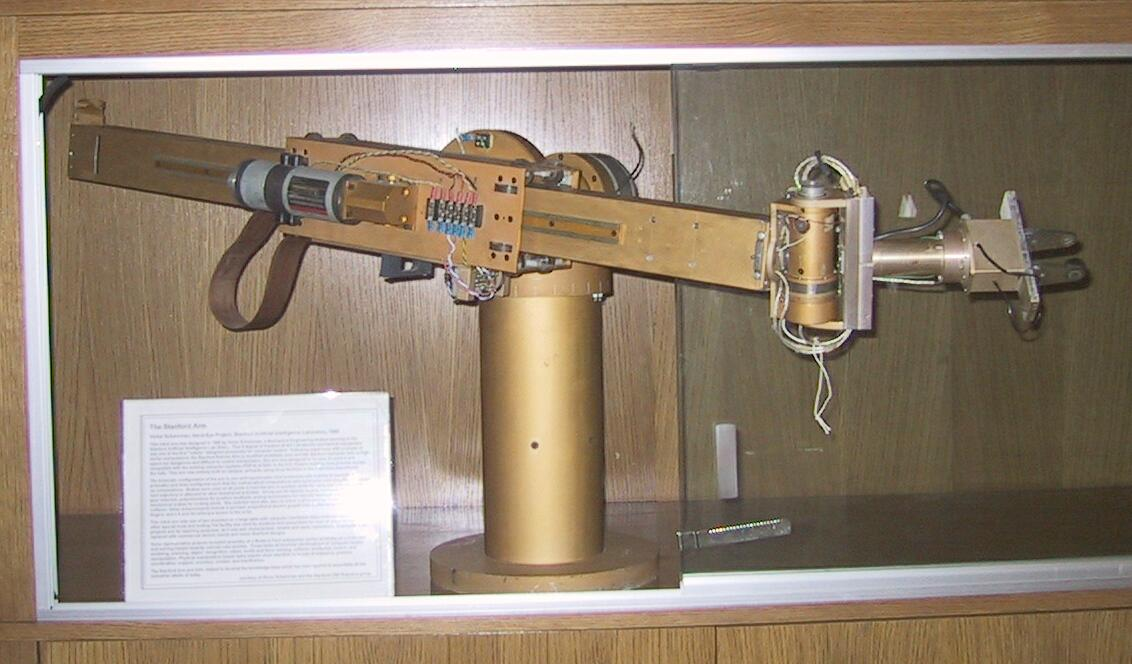
\includegraphics[width=0.50\linewidth ,height=0.4\columnwidth]{figures/StanfordArm.jpg} \,\,
 		&
 		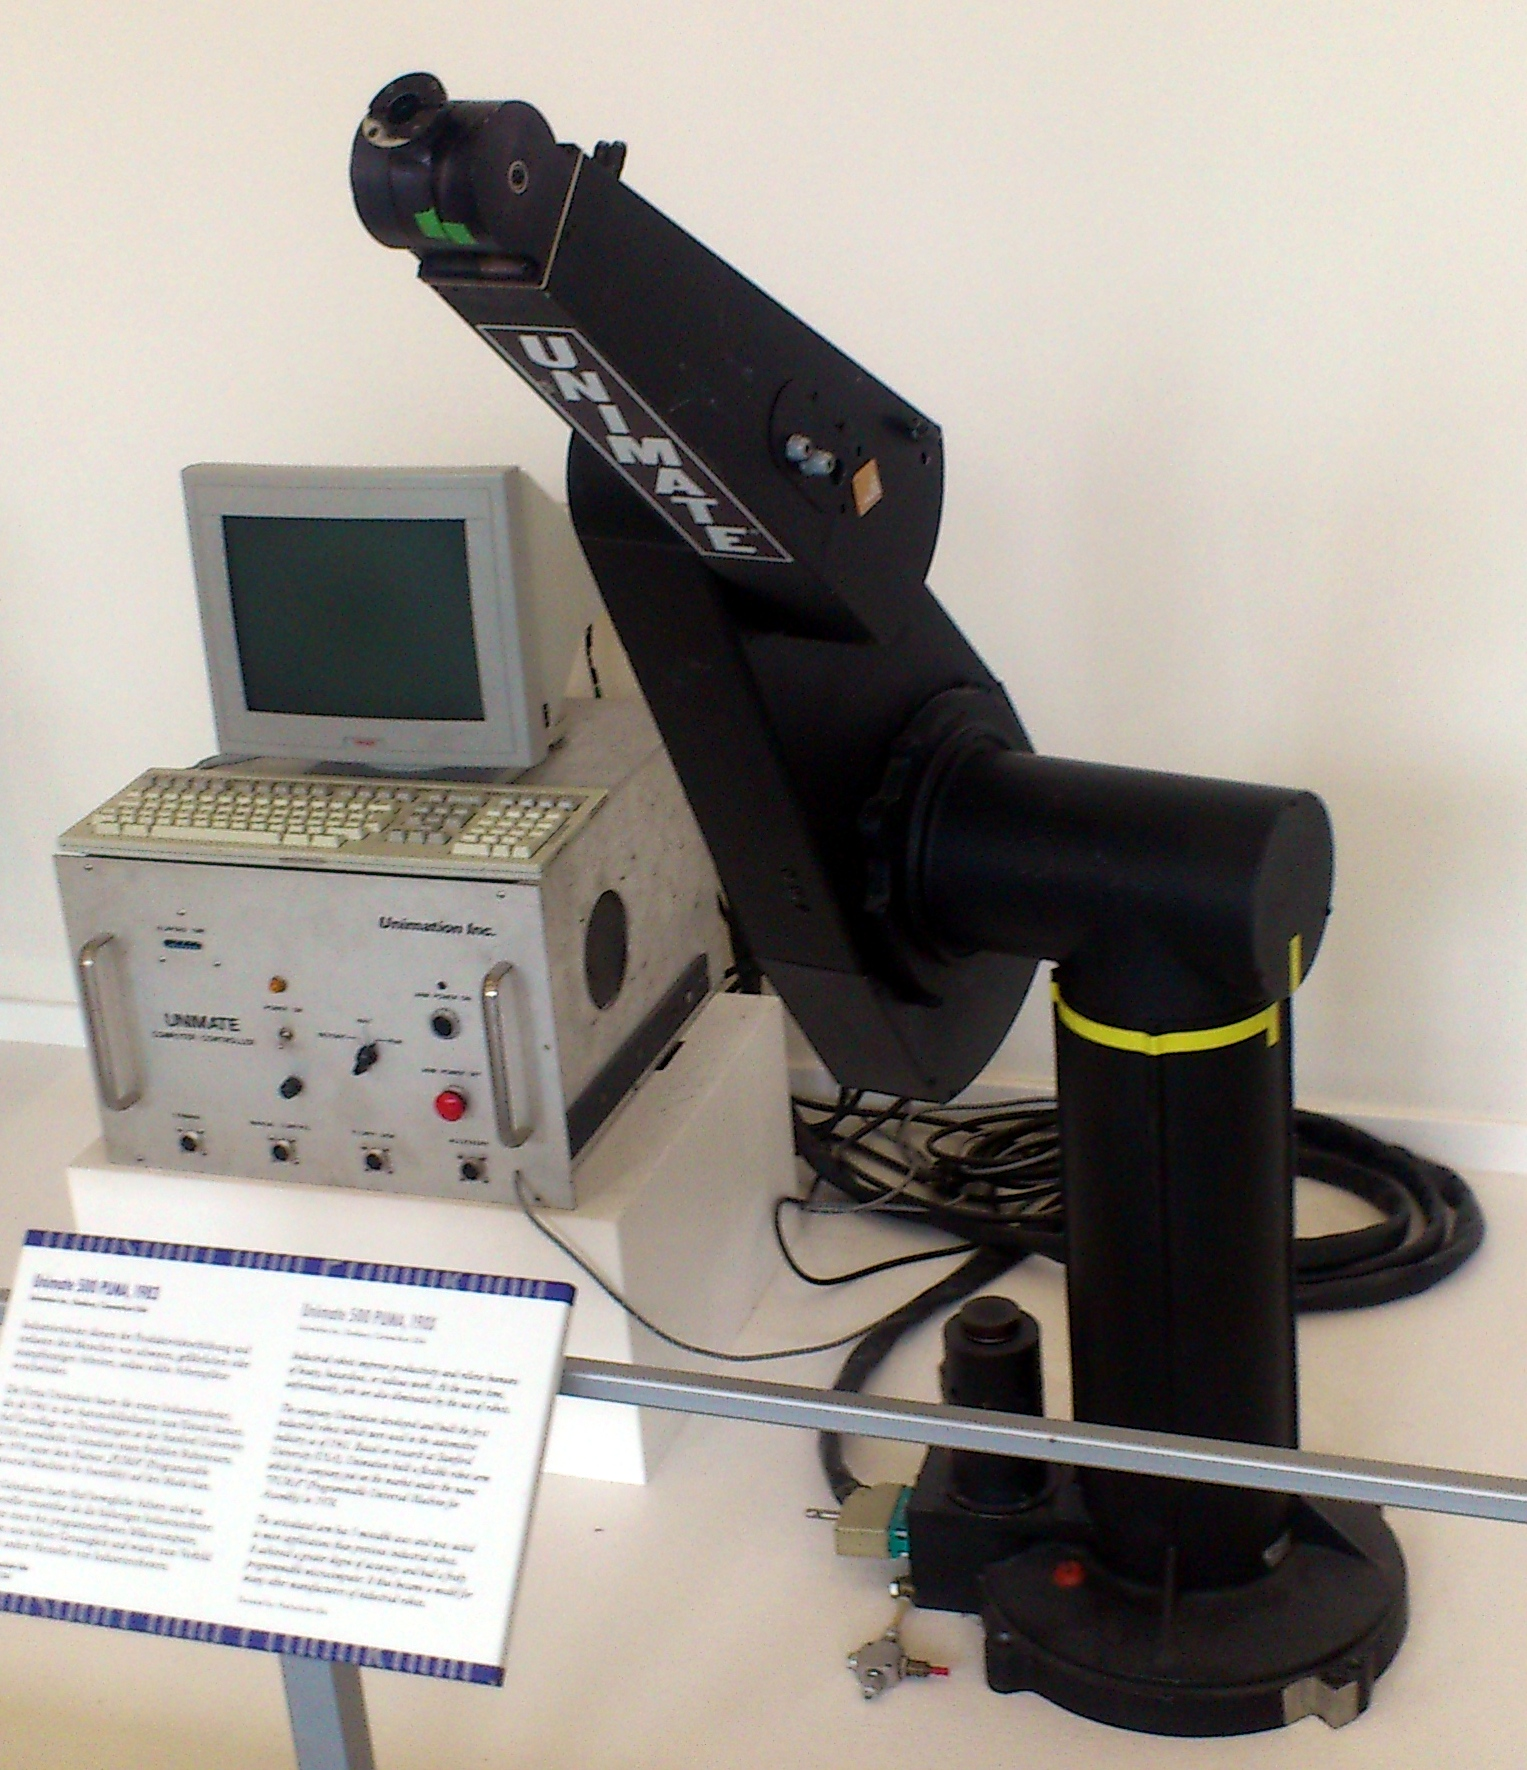
\includegraphics[width=0.48\columnwidth,height=0.4\columnwidth]{figures/PUMA.jpg}
 	\end{tabular}
 	\caption{Early serial kinematic chain robot manipulators. \textit{Left:} The Stanford Arm Serial Manipulator, 1969. \copyright Infolab, Stanford University. \textit{Right:}  The PUMA robot arm. Reprinted from Wikipedia.}
 	\label{fig:robot_arms}
 \end{figure}
 %
A kinematic chain is a form of a \textit{mechanism}. A ``\textit{mechanism can be interpreted as a means of transmitting, controlling, or constraining relative movement}"~\cite{HuntBook1977}. The term \textit{kinematics} is generally used to describe the motion of a rigid body in space. It also applies to the motion of a semi-rigid or a  completely soft robot in space.  The rigid, semi-rigid or completely soft kinematic systems that allow a body to exhibit motion under a/some controlled motion of its freedom in space with respect to a fixed base frame are what we describe in this module.
 %

\begin{figure}[tb!]
	\centering
	\begin{tabular}{@{}c@{}c@{}}
		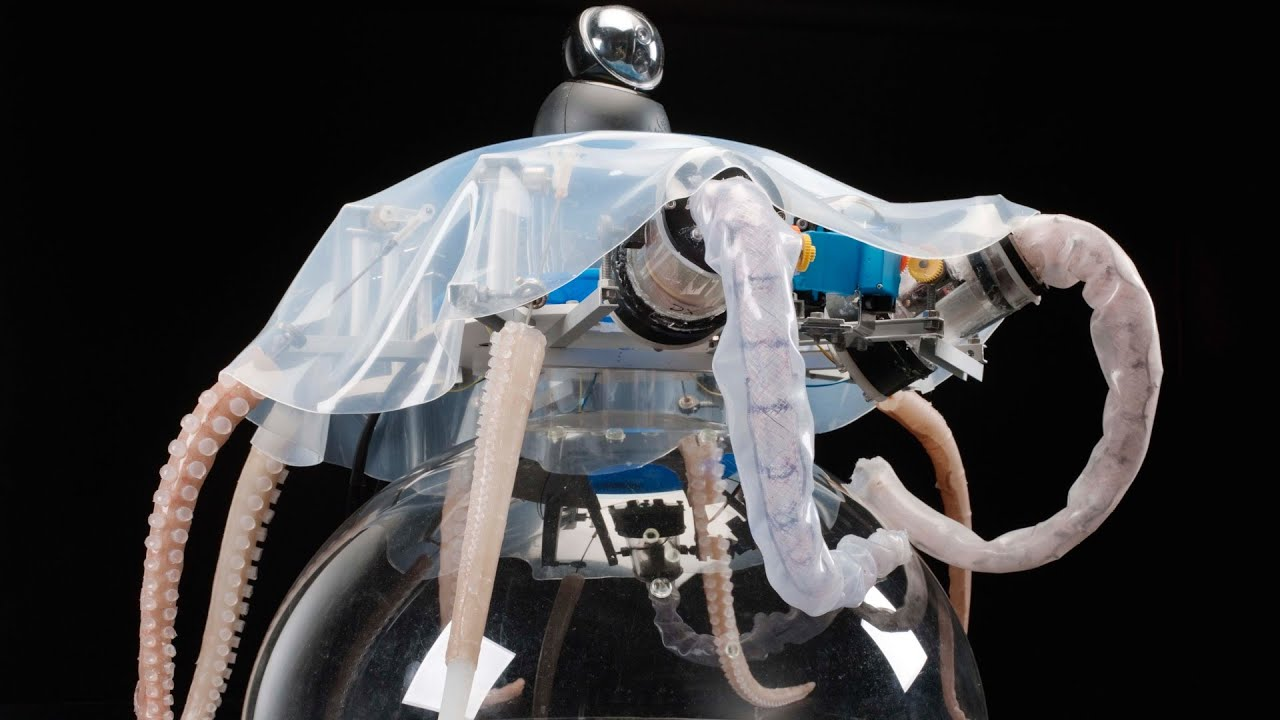
\includegraphics[width=0.50\linewidth ,height=0.4\columnwidth]{figures/octopus.jpg} \,\,
		&
		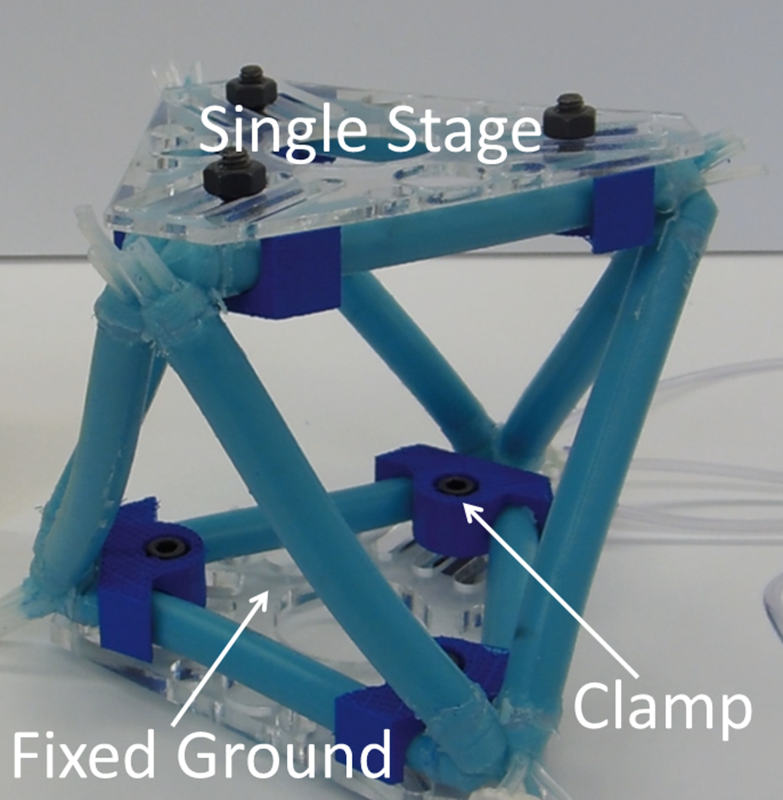
\includegraphics[width=0.48\columnwidth,height=0.4\columnwidth]{figures/soft_parallel.png}
	\end{tabular}
	\caption{Soft Robot Manipulators \textit{Left:} An octopus inspired soft robot. Robots classified under muscular hydrostats. \copyright Cecilia Laschi. \textit{Right:} A soft parallel robot manipulator ~\cite{hopkins2015synthesis}.}
	\label{fig:soft_robots}
\end{figure}

 \section{Robots Components}
 
The joints of a robot can be \textit{revolute} or \textit{prismatic}. Revolute joints allow rotation about a fixed axis between two or more links while prismatic joints allow a linear motion about an \textit{axis} -- which is between two links. Symbolically, the revolute joint is denoted by $R$ while the prismatic joint is denoted by $P$. By this logic, it follows that a robot made up of three links that are connected by a prismatic joint would be characterized as a $PPP$ arm, while a three link arm whose links are all connected by three rotary joints would be denoted as an $RRR$ arm. 
 
 A mathematical way to abstract the interconnection between the links of a robot arm is to denote the axis of rotation or the axis of translation by $z_i$ for the joint that connects link $i$ to link $i+1$. When we characterize the robot's motion, it often helps to work in a so-called \textit{generalized coordinate}. Now consider a rigid body such as a link of a robot arm for example. This link contains myriads of particles, with each particle having its own position and orientation in the world. How can we describe the motion of this rod given its infinitely many particulate matter? For rigid bodies, classical mechanics comes to the rescue. As such, for a revolute joint of a rigid robot manipulator for example, the generalized coordinate is often the \textit{joint angle} $\theta$, while for a prismatic joint it is the link length $d$ -- representing the relative displacement between adjacent links. When the body we speak of is a continuum, the motion of each particle within a link needs to be accounted for. In such scenarios, researchers often work with a so-called a \href{http://web.mit.edu/hyperbook/Patrikalakis-Maekawa-Cho/node25.html}{Frenet-Serret} frame that models  a curve on the soft robot's surface -- with or without torsion. This simplifies the dynamics and kinematics of the system and the specification of these generalized coordinates uniquely determines the position of all the particles (in a material sense for a rigid system) that make up the robot. For more examples on parameterizing soft robots, please look through some of the following references: \cite{Ogunmolu15CASE}, \cite{Hannan2000} \cite{Ogunmolu16CASE}, \cite{Renda2018ICRA}, \cite{ShepherdMultigait}, \cite{Hannan2003}, \cite{Ogunmolu17IROS}, \cite{Laschi15NeuNet}, \cite{Ogunmolu19RALI}, \cite{Renda2014Cosserat}, \cite{Ogunmolu19RALII}, \cite{OgunmoluThesis}.
% 
 
 \section{Robot Spaces, Geometries, and Classifications}
 
 The location of a robot in the world is described by its \textit{configuration}. This configuration specifies the positions of all points of the robot. While the coordinates of these points may be multiple over a continuous range of real numbers, the smallest number of independent variables of these real-valued coordinates needed to represent the robot configuration are the \textit{degrees of freedom} of the system.  In general, a \textit{free rigid body} has six degrees of freedom. The motion of the robot could be about a translation or rotary axis. The $n$-dimensional space that contains all the possible configurations of the robot is the \textit{configuration space} (or \textit{C-space}) of the robot. The configuration of the robot is expressed by a point in its C-space. 
 
 A manipulator with more than 6-\dof is said to be \textit{kinematically redundant}. %In general, the total number of the degrees of freedom of a \textit{rigid body} in space cannot exceed 6-\dof~\cite{Merlet2015}. 
 The set of variables that together with a description of the manipulator's dynamics and future inputs that determines the future transient response of the manipulator is the \textit{state} of the robot, while the set of all possible states is referred to as the \textit{state space}. For a rigid robot manipulator for example, the material and referential description alone is sufficient to describe the dynamics, which are Newtonian in nature. For such systems, the state may be specified by the joint variables $\{q, \dot{q}\}$ signifying the joint angles and joint velocities. For continuum systems, such representations are often inadequate. A popular method is to introduce a Frenet-Serret (you can read more about F-S frames in the link included earlier) frame on the body of the soft robot (SoRo) and characterize the state space based on the three parameters \ie $\{\mathcal{K}, l, \alpha\}$ that characterize the kinematic motion of the body viz., curvature of an arc projected on the SoRo's body, $\mathcal{K}$, the arc's length, $l$, and the angle subtended by a tangent along that arc, $\alpha$.
 
 \section{Characterization of Kinematic Geometry}
 %
 As mentioned earlier, disassociated from the dynamics (\ie forces, torques and such) of a body, that which deals with the displacements, or movements of a body relative to another within a mechanism is termed the \textit{kinematics}. The displacement could be linear, angular -- and in combination with the derivatives with respect to time of such displacements viz., velocities, accelerations, and hyper-accelerations all are part of the kinematics of a body. The other branch of \textit{dynamics}, called \textit{kinetics}, determines the forces, torques, energy, momenta, inertia, equilibrium and dynamic stability of the system and that is treated in a separate module in this course.
 
 \subsection{Kinematic Geometries}
 %
 Kinematic geometry deals only with the \textit{displacements} of a system in the first and simplest segment of kinematics.  In general, the use of time as a variable is shunned upon since the displacements we intend to carry out may be performed as fast as user wishes in their implementation.  For the rest of this subsection, by kinematics, we shall mean the displacement of rigid bodies or ``the solid geometry of relatively moving bodies". 
 
 The majority of robot arms (at least today) have their actuators (or joints) connected in series along an \textit{anthropomorphic} arm, with each joint being either at or associated with a single \dof in the robot arm. 
 %
\begin{figure}[tb!]
	\centering
	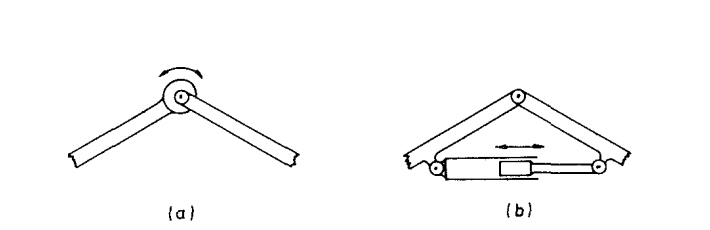
\includegraphics[width=\columnwidth]{figures/arms_hunt.png}
	\caption{Schematic description of in-series-actuated robot arms: (a) rotary joint actuated ``about" the hinge (b) prismatic joint actuated ``across" a hinge. Reprinted from \cite{Hunt1983}.}
	\label{fig:arms_schematic}
\end{figure}
%
\autoref{fig:arms_schematic} describes the two major ways rigid links are actuated today. From a geometric point of view, both types of actuation in \autoref{fig:arms_schematic} serve the same purpose, which is to control the rotation of the joint. However, when we are interested in controlling ``pure translation" such as sliding between links, non-pivoted linear actuators are used on their own. 


\subsection{Open Kinematic Chains}

When the links are serially connected to one another and there is no link that connects the base link to the tool frame, the robot is said to be in-series actuated. Series-jointed links have a major disadvantage, namely that they accumulate errors from shoulder out to end-effector and they suffer from a lack of rigidity. In order to eliminate their inherent load-dependent error, manufacturers typically stiffen them. However, this stiffening process increases the mass of the arm such that greater demand is placed on the actuation system. Some manufacturers employ  a compensated actuation or sophisticated control techniques in order to  overcome the load-dependent errors. 
%
\begin{figure}[t!]
	\centering
	
\includegraphics[scale=.1, width=.4\columnwidth]{figures/Staubli.jpg}
	\caption{The Staubli 6-DOF Arm is an example of a Spherical Manipulator. Reprinted from DirectIndustry's Webpage.}
	\label{fig:staubli}
\end{figure}

Examples of in-series actuated mechanisms is the \textit{spherical robot} (see \autoref{fig:scara_bot}), where a succession of the robot segments are linked to the predecessors by revolute joints. By actuating each of the $n$ joints we can control the $n$ degrees of freedom of the end-effector. 
%
\begin{figure}[b!]
	\centering
	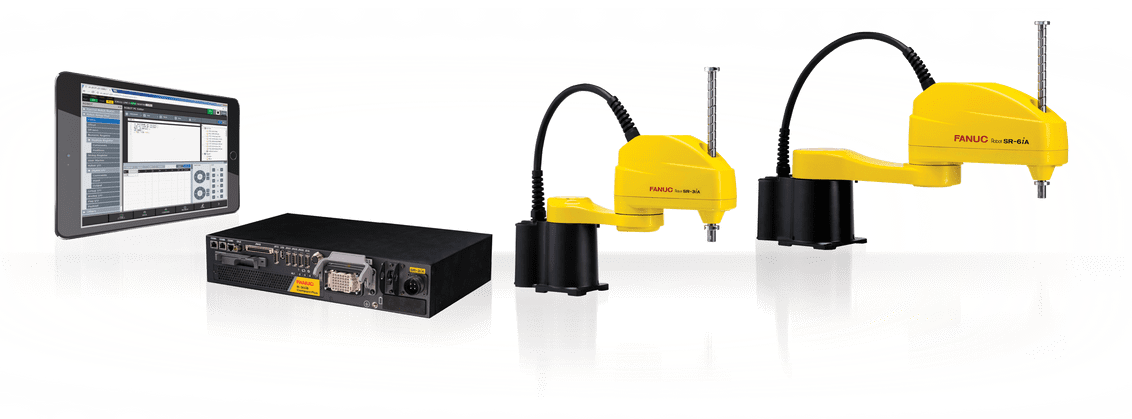
\includegraphics[width=\columnwidth]{figures/Scara.png}
	\caption{The SCARA Arm. \copyright Fanuc America.}
	\label{fig:scara_bot}
\end{figure}
%
The SCARA robot, shown in \autoref{fig:scara_bot} is an example that allows the control of the end-effector based on the geometry of the previously connected links. 

It is ideally desirable to keep the load-to-mass ratio of a robot as minimum as possible whilst preserving positioning accuracy. This is so as to preserve two important properties of the robot: repeatability (\ie the maximum distance between two positions of the end-effector reached for the same desired pose from different starting positions),  and absolute accuracy (\ie distance between the desired and actual position of the end-effector) respectively. Positioning accuracy is a function of the deformation of flexure -- typically not accounted for by the robot's internal sensors -- and the absolute accuracy. The absolute accuracy is a function of the sensors at the manipulator joints, the clearance for the drive, flexure of links, and geometric accuracy of link orientations inter alia. When geometric constraints are violated (take a small error in the perpendicularity between successive links of a spherical arm, for example), large errors are bound to occur in the vertical motions so that such errors must be accounted for during manufacture. The conventional approach to overcoming this currently is for manufacturers to stiffen the robot's links. However, stiffening the links is tantamount to overall heavier mass, which in turn means the manipulator experiences higher inertia, centrifugal and Coriolis forces -- these complicate motion planning for complex trajectories.  

As we close this part of the module, bear in mind that open kinematic chains are governed by inertia and centrifugal forces -- forces that exist on different scales. For example, inertia forces are a function of the square of the link lengths while frictional forces are not affected by the such dimensions. As such, serial robots cannot be scaled down to a micro level as inertia forces would be reduced while frictional forces would remain unchanged. It is not surprising that these attributes listed make serial manipulators exhibit poor positioning accuracy. 

\subsection{Closed-loop Kinematic Chains}
 
 When the number of links connected to a joint (the \textit{connection degree}) is more than 2, we have a closed-loop kinematic chain. Closed-loop kinematic chains resolve the accuracy problems of open-loop chains by mechanically distributing the load on the links: they link the end-effector to the ground by a set of links that support only a fraction of the load. While theoretical works that envisioned parallel mechanisms have been in existence since 1645~\cite{Merlet2015}, the Stewart~\cite{Stewart1965} and Gough~\cite{Gough1957} platforms are the original designs of closed-loop chains on record. 
 %
 \begin{figure}[tbph!]
 	\centering
 	\begin{tabular}{@{}c@{}c@{}}
 		\includegraphics[width=0.50\linewidth ,height=0.4\columnwidth]{../../../Papers/PhDThesis/figures/GoughPlatform.png} \,\,
 		&
 		\includegraphics[width=0.48\columnwidth,height=0.4\columnwidth]{../../../Papers/PhDThesis/figures/GoughPlatformNow.jpg}
 	\end{tabular}
 	\caption{Stewart-Gough Platforms \textit{Left:} The 1954 Octahedral hexapod of the original Gough platform. \textit{Right:} The retired platform from Dunlop tires in 2000. Picture courtesy of Parallemic.org.}
 	\label{fig:stewart_gough}
 \end{figure}
%
The mechanical arrangement of the links of the platform help with the load-to-mass ratio: the manipulator mass is reduced, and the disturbing effects of the Coriolis forces decreases. Albeit, these manipulators typically have a smaller workspace.
Formally, we define a \textit{generalized parallel manipulator} as a closed-loop kinematic chain mechanism whose end-effector is linked to the base by many independent kinematic chains~\cite{Merlet2015}.
 
 \section{Freedom and Structure in Mechanisms}
 
 Early on, we briefly defined what constitutes the degrees of freedom of a rigid body. We will now systematically analyze how to determine the mobility of a mechanism given its \textit{kinematic pairs}, linkages and freedoms.
 
 \subsection{Freedom, Connectivity and Mobility}
 
 For every \textit{kinematic pair}\footnote{Bonus homework: Research what is a kinematic pair and produce a one-page written report.}, there exists a characteristic number of the degrees of freedom that characterize its mobility.  If a kinematic pair has elements that touch at a single point, we would have five degrees of freedoms -- two of which would be translatory and three rotary. A kinematic pair whose elements always touch along a line or a curve has four or fewer degrees of freedom, or for short, freedom (see \autoref{fig:kinematic pair}).
%
\begin{figure}[tb!]
	\centering
	%\emptybox{4cm}
	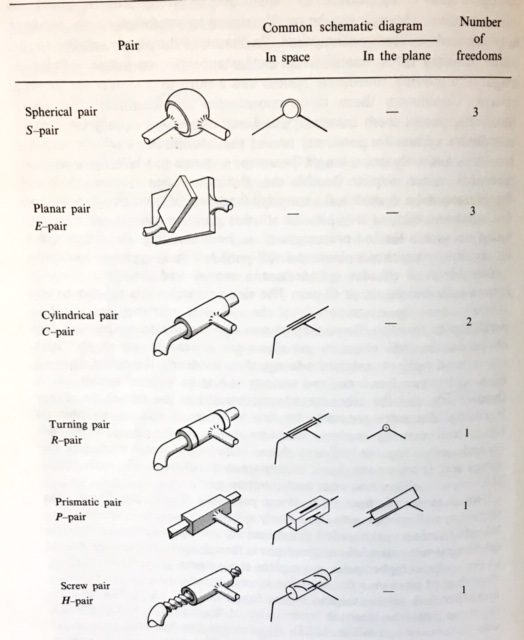
\includegraphics[width=.46\columnwidth, height=.5\columnwidth]{figures/kinematic_pair2.jpg}
	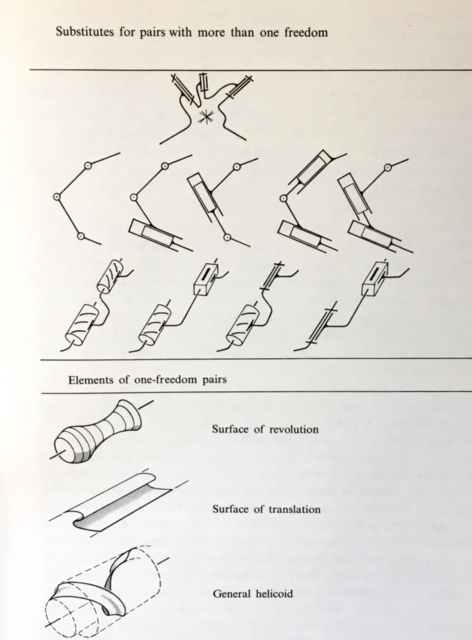
\includegraphics[width=.46\columnwidth, height=.5\columnwidth]{figures/kinematic_pair.jpg}
	\caption{The Lower Kinematic Pairs. Reprinted from \cite{HuntBook1977}.}
	\label{fig:kinematic pair}
\end{figure}

However, in mechanisms, we are more concerned about the relative motion between objects in the mechanisms that do not directly touch one the other. In such systems, what we do is consider the freedom that is contributed by each of the several kinematic pairs that connect them. For the popular four bar linkage, for example (see ~\cite{MurrayBook}), the four $R$-pairs on the two connectivity-links 2 and 4 complete a \textit{coupling} or \textit{connection} between 1 and 3. This is said to have a connectivity of $1$, typically written as $\mathscr{C}_{13}=1= \mathscr{C}_{31}$. Note that here, all connectivities are the same , and $\mathscr{C}_{ij} = 1$, for $i \neq j$ and $i,j=1,2,3,4$. Now, suppose that the $R$ pairs are replaced by spherical, or for short, $S$ pairs, then we have an additional so-called \textit{spin-freedom} about the $SS$ axis (see figure \autoref{fig:four_bar})
%
\begin{figure}[tb!]
	\centering
	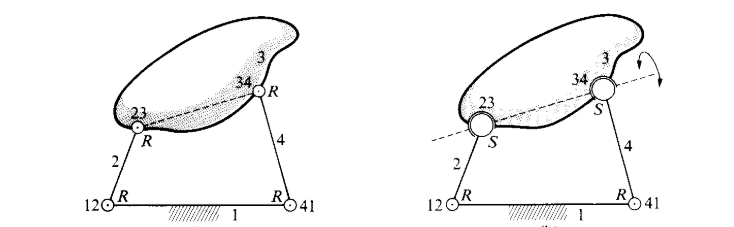
\includegraphics[width=\columnwidth]{figures/four-bar-linkage.png}
	\caption{The planar $RRR$ linkage, (\textit{left}) is modified in (\textit{right}) to allow spatial spin-movement of the coupler 3; the connectivity $\mathscr{C}_{13}=2$). Reprinted from ~\cite{HuntBook1977}.}
	\label{fig:four_bar}
\end{figure}
%
so that $\mathscr{C}_{13}=2$. In any case, $\mathscr{C}_{12}=\mathscr{C}_{13}=\mathscr{C}_{43} = 2$.

Related to the concept of connectivity and more popular in literature is the concept of \textit{relative mobility} or simply \textit{mobility}.  The mobility, $\mathfrak{M}$, is usually referred to as the number of \textit{degrees of freedom} of a mechanism. To specify the independent variables needed to determine all the relative locations of the complete members of a mechanism with respect to one another, we typically use the \textit{mobility criterion}. As such, we would have the kinematic chain of the left inset of \autoref{fig:four_bar} having $\mathfrak{M}=1$ since only an angle between the elements of any of the four kinematic pairs is required so as to prevent all relative movement. However, for the $RSSR$ mechanism on the right of \autoref{fig:four_bar}, the mobility would be $\mathfrak{M}=2$ since member $3$ has a spin-freedom.

\begin{tcolorbox}[title=Determining Degrees of Freedom]
	\textit{Screw Coordinates} are better suited -- from a kinematic standpoint, at any rate -- to determine the general and impartial location of a rigid body.
\end{tcolorbox}

\subsection{Constraints and Freedoms}
%
In rigid body kinematics, it is a given that the freedoms of a \textit{free rigid body} is $6$. But how is this determined? Suppose we have six homogeneous \textit{screw coordinates} (to be introduced shortly) $x_1, x_2, \ldots, x_6$, we find that the body is fixed when values are attached to all six of them. However, the physical constraining system to which the body is subjected is not likely to have for every constraint exactly one corresponding independent screw coordinate. For every constraint in the system, there is an influence on each of the six coordinates. For every independent constraint, a freedom of the body is suppressed so that the six independent constraint-equations $f_i(x_1, x_2, \ldots, x_6)=0, \, i = 1, 2, \ldots, 6$ must all be simultaneously satisfied. We define the \textit{condition} as the constraint equation that describes a particular constraint algebraically. As the constraints are progressively relaxed, the corresponding constraint-equations are struck out one after another, so that the body acquires one, two, $\ldots$, degrees of freedom, until the body is completely free with no constraints or equations and we end up with six freedoms. Suppose the number of freedoms is $f$ and the number of \textit{unfreedoms} or constraints is $u$, it turns out that 
%
\begin{equation}
	u + f = 6.
	\label{eq:unfreedom}
\end{equation}

\subsection{The Mobility Criterion}

For $g$ working joints between a total of $n$ bodies, the number of relative degrees of freedom can be identified with the relative mobility of the system of bodies, described as 
%
\begin{align}
	\mathfrak{M} = 6(n-1) - \sum_{i=1}^{g} u_i
	\label{eq:mob_bodies}
\end{align}
%
where the summation term aggregates over all individual unfreedoms. Plugging \eqref{eq:unfreedom} into  \eqref{eq:mob_bodies}, we have 
%
\begin{align}
\mathfrak{M} = 6(n-1) -\sum_{i=1}^g 6 + \sum_{i=1}^{g} f_i
\end{align}
%
or 
%
\begin{align}
\mathfrak{M} = 6(n - g - 1) + \sum_{i=1}^{g} f_i.
\label{eq:mob_cond_gen}
\end{align}

Equation \eqref{eq:mob_cond_gen} is termed the general mobility criterion. It is attributed to Gr\"ubler (1908 and 1917), and independently to Kutzbatch (1929). In this module, we will generally call it the Gr\"ubler-Kutzbach's mobility criterion. When there are independent kinematic chains within the body of concern, it is sometimes more convenient to write \eqref{eq:mob_cond_gen} as 
%
\begin{align}
	\mathfrak{M} = \sum_{i=1}^g f_i - 6c
	\label{eq:mob_loop}
\end{align}
%
with $c$ being the number of independent chains. 

There are exceptions to the Gr\"ubler-Kutzbach's mobility criterion such as when we have planar or spherical mechanisms. Take the four-bar linkage for example. There are four freedoms to the kinematic pairs, yet patently it has a mobility of $\mathfrak{M}=1$, and not $\mathfrak{M}=-2$ as \eqref{eq:mob_loop} would have us so determine it.  This is because for planar and spherical mechanisms, the number of freedoms is not six as in \textit{general} space, but three. Therefore, we write out the special version of \eqref{eq:mob_cond_gen} as 
%
\begin{align}
\mathfrak{M} = 3(n - g - 1) + \sum_{i=1}^{g} f_i.
\label{eq:mob_cond_planar}
\end{align}
%
This special nature of \eqref{eq:mob_cond_planar} arises because the joints' freedoms are not independent in planar motion, because the axes of the turning pairs are all directed parallel to one another, any prismatic pair being perpendicular to them. For spherical motions, the turning axes co-intersect at a single point.

\begin{homework}
	Read up on the common kinematic arrangements in Section 1.3 of~\cite{SpongBook} and produce a 2-page single-spaced summary report. Your report must not contain diagrams but feel free to do as much analysis of the configurations of the various kinematic arrangments that are mentioned. \newline
	\begin{itemize}
%		\item 
		%
		\item Using the mobility condition, determine and explain why the SCARA robot of \autoref{fig:scara_bot} has the number degrees of freedom that you find.
		%
		\item For the mobile manipulator we are using in this course, analyze the connectivities and freedoms of the kinematic pairs in the mechanism. In addition, determine the freedom of the overall mechanism and write out the mobility criterion.
		%
		\item With the \textit{{Gr\"ubler-Kutzbach's} mobility condition} that we have learned, analyze the mobility criteria of the mechanism of \autoref{fig:para_mech}. Hint: This mechanism is made up of two chains: chains $A_3\, B_3\, B_1\, A_1$ and $A_2\, B_2\, B_4\, A_4$, and there is a fixed distance between the $U$-joints, $A_2\, A_3$ as well as $A_1, A_4$.
		%
	\end{itemize}
\end{homework}


\begin{figure}[tb!]
	\centering
	\begin{tabular}{@{}c@{}c@{}}
	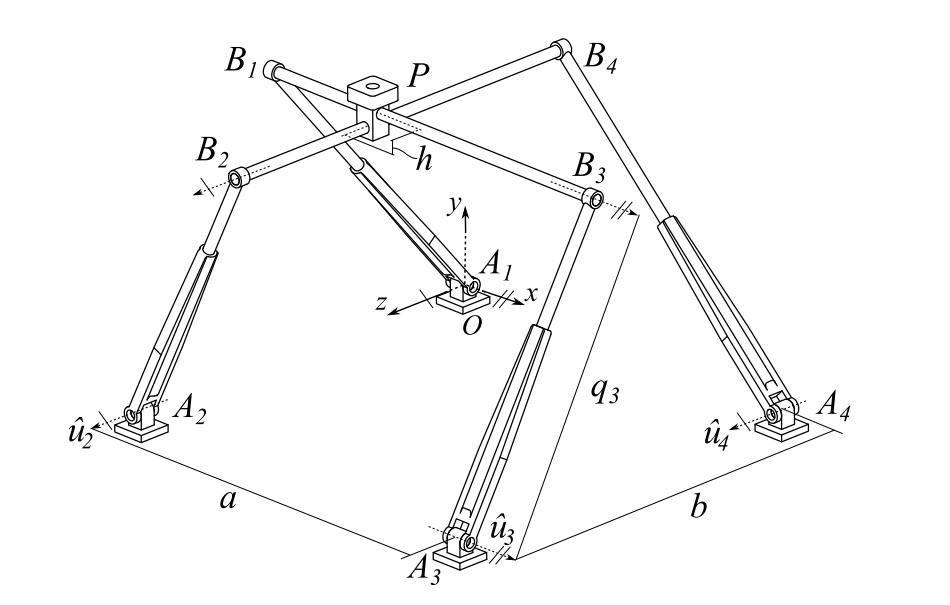
\includegraphics[width=0.50\linewidth ,height=0.4\columnwidth]{figures/parallel_translational.png} \,\,
	&
	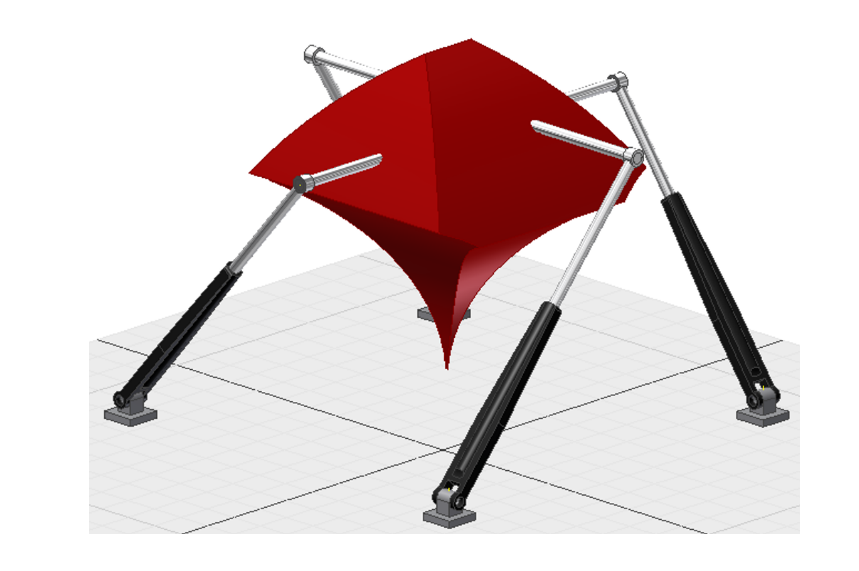
\includegraphics[width=0.48\columnwidth,height=0.4\columnwidth]{figures/parallel_translational_workspace.png}
	\end{tabular}
	\caption{\textit{Left}: A Parallel Planar Robot Mechanism. \textit{Right:} Workspace of the mechanism.}
	\label{fig:para_mech}
\end{figure}